\documentclass[../kl10.tex]{subfiles}
\graphicspath{{\subfix{../images/}}}

\begin{document}

\section{Eine Trennung geht immer - man braucht nur genug Druck}

Wird eine Lösung mit dem reinen Lösungsmittel vermischt, führt dies zu einer gleichmäßigen Verteilung des gelösten Stoffes. 
Wird zwischen den beiden Flüssigkeiten vor ihrer Mischung eine Membran installiert, welche nur das Lösungsmittel, aber nicht den gelösten Stoff durchlässt, kann kein kompletter Konzentrationsausgleich zwischen den zwei Flüssigkeiten beobachtet werden. Dies liegt daran, dass es für den gelösten Stoff nicht möglich ist, die Membran zu passieren und so die Konzentration auszugleichen. Stattdessen baut sich ein sogenannter Osmotischer Druck auf, welcher einen Teil des Lösungsmittels in die Lösung „drückt“. 
Der Osmotische Druck $\Pi$ kann äquivalent zum Gasdruck $p$ mit dem \textsc{van-’t-Hoffschen} Gesetz berechnet werden:
$$\Pi \cdot V =n \cdot R \cdot T $$
Dieser Druck kann auch auf die Lösung ausgeübt werden, sodass sich keine Volumen- und damit Konzentrationsänderung ergibt. 
\enumaufgabe{\operator{Berechne}, wie hoch der osmotische Druck einer Zuckerlösung mit der Konzentration $c = 2,000\cdot 10^{-3}\ \si{\frac{mol}{L}}$ bei Standardbedingungen (\SI{0}{\celsius}, \SI{1}{\bar}) ist.}

\solution{$$\Pi = c \cdot R \cdot T = 2,000 \cdot 10^{-3} \thinspace \mathrm{M} \cdot 8,3145 \thinspace \mathrm{(J/K\cdot mol)} \cdot 273,15 \thinspace \mathrm{K}$$$$=2,000 \thinspace \mathrm{mol/m^3} \cdot 8,3145 \thinspace \mathrm{J/(K\cdot mol)} \cdot 273,15 \thinspace \mathrm{K}=4,542 \cdot 10^3 \thinspace \mathrm{Pa}$$
1,5 P.}{2cm} 
Neben Lösungen aus zwei Komponenten (Lösungsmittel mit gelöstem Stoff) können auch Lösungen von ionischen Verbindungen einen osmotischen Druck ausüben. Um die erhöhte Teilchenanzahl bei gleicher Konzentration zu berücksichtigen, wird der \textsc{van-’t-Hoff}-Faktor $i$ der Gleichung zugefügt: 
$\Pi \cdot V =i \cdot n \cdot R \cdot T $
Dabei ist $i$ der Quotient aus der Stoffmenge an gelösten Ionen geteilt durch die Stoffmenge des zugefügten Salzes: $$i= \frac{\sum{n_\text{gelöst}}}{n_0}$$
\enumaufgabe{\operator{Berechne} den osmotischen Druck einer \ce{CaI2}-Lösung mit der Konzentration $c = 5,000\cdot 10^{-3}\ \si{\frac{mol}{L}}$ bei Standardbedingungen (\SI{0}{\celsius}, \SI{1}{\bar}).}

\solution{
$$\Pi = i \cdot c \cdot R \cdot T =3 \cdot 5,000 \thinspace \mathrm{mol/m^3}\cdot 8,3145 \thinspace \mathrm{J/(K\cdot mol)} \cdot 273,15 \thinspace \mathrm{K}=3,407\cdot 10^4 \thinspace \mathrm{Pa} $$
1,5 P.}{2cm}

Durch Messung des osmotischen Druckes können Informationen über die vorliegende Lösung gewonnen werden, wie beispielsweise der Grad der Dissoziation. Betrachte das Folgende Dissoziationsgleichgewicht:

\begin{center}
    \ce{HA <=> H^{+} + A^{-}}
\end{center}

Der Dissoziationsgrad $\alpha$ beschreibt, welcher Anteil eines Stoffes in der Lösung dissoziiert vorliegt und ist wie folgend definiert: $$\alpha=\frac{c(\ce{A-})}{c(\ce{HA})_0}$$

\newpage

\enumaufgabe{\operator{Berechne} den Dissoziationsgrad $\alpha$ einer  \SI{0,1000}-molaren \ce{HA}-Lösung, welche unter Standardbedingungen (\SI{0}{\celsius}, \SI{1}{\bar}) einen osmotischen Druck von \SI{4e5}{\pascal} ausübt. \\
Hinweis: Das Autoprotolyse des Wassers kann vernachlässigt werden.}

\solution{
$$\alpha=\frac{[\ce{A-}]}{c_0}$$
Aus Hinweis starker Säure und 0,1 M folgt $[\ce{A-}]=[\ce{H+}]$
$$c_{\mathrm{ges}}=[\ce{HA}]+[\ce{A-}]+[\ce{H+}]=c_0+[\ce{A-}]=c_0\cdot(1+\alpha)\qquad \mathrm{1 P.}$$
$$\Pi=c_{\mathrm{ges}}RT\qquad \mathrm{1 P.}$$
$$c_{\mathrm{ges}}=\frac{\Pi}{RT}=\frac{4\cdot10^5\thinspace\mathrm{Pa}}{8,3145 \thinspace \mathrm{J/(K\cdot mol)} \cdot 273,15 \thinspace \mathrm{K}}=0,1761\thinspace\mathrm{M}\qquad \mathrm{1 P.}$$
$$\alpha=\frac{c_{\mathrm{ges}}}{c_0}-1=\frac{0,1761\thinspace\mathrm{M}}{0,1000\thinspace\mathrm{M}}-1=0,761\qquad \mathrm{1,5 P.}$$
Insg. 4,5 P.}{6cm}

Bei einem Versuchsaufbau (\autoref{Skizze1}) wird ein großes Gefäß in der Mitte durch eine Membran in zwei identische Bereiche geteilt. In der linken liegt destilliertes Wasser, in der rechten die Zuckerlösung aus Teilaufgabe a) vor. Der osmotische Druck kann durch den Fluss von Lösungsmittel und dem einhergehenden Anstieg bzw. Absenken der Lösungen in den dünnen Stäben erreicht werden. Der durch Höhenunterschied in einer Lösung erzeugte Druck lässt sich wie folgt berechnen: $$p = \rho \cdot g \cdot h$$
Dabei beschreibt $\rho = 0,9998 \thinspace \mathrm{g/cm^3}$ die Dichte der Lösungen, $g = 9,807 \thinspace \mathrm{m/s^2}$ die Erdbeschleunigung und $h$ den der Höhenunterschied. 

\begin{figure}[H]
    \centering
    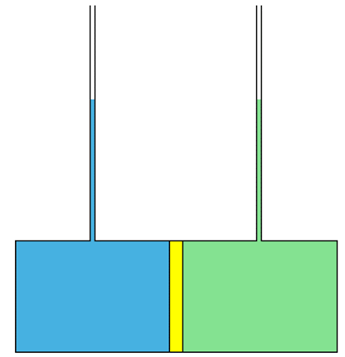
\includegraphics[width=0.4\textwidth]{2024/Abbildungen/Umkehrosmose/U_Rohr.png}
    \caption{Skizze zur Umkehrosmoseanlage}
    \label{Skizze1}
\end{figure}

\newpage

\enumaufgabe{\operator{Berechne}, um welche Höhe die Lösung in der rechten Röhre ansteigen muss, um den osmotischen Druck auszugleichen. \\Falls du Teilaufgabe a) nicht gelöst hast, rechne mit $4,200 \cdot 10^3 \thinspace \mathrm{Pa}$}
\solution{
$$\Pi=p\qquad \mathrm{0,5 P.}$$
$$\Pi = \rho \cdot g \cdot h$$ 
da auch andere Seite gleichermaßen sinkt Faktor 2 (0,5 P.):\\
$$ h = \frac{\Pi }{2 \rho \cdot g } = \frac{4,542 \cdot 10^3 \thinspace \mathrm{Pa}}{2 \cdot 999,8 \thinspace \mathrm{kg/m^3} \cdot 9,807 \thinspace \mathrm{m/s^2}} = 0,2316   \thinspace \mathrm{m}\qquad \mathrm{1,5 P.}$$
Ergebnis mit Ersatzannahme: $0,2142\ \si{m}$\\
Insg. 2,5 P.}{6cm}


\enumaufgabe{\operator{Begründe} kurz, ob im Experiment diese Höhe eher über- oder unterschritten wird.}

\solution{
Die Membran ist nie 100\thinspace\% undurchlässig, sodass der Konzentrationsunterschied etwas ausgeglichen wird. Die Konzentration im Gefäß ändert sich bei dem Vorgang, wodurch der osmotische Druck mit Konzentrationsausgleich sinkt. Zudem ist das Gesetz nur eine Näherung und unter Einbezug der Aktivität würde der Druck auch geringer sein.\\
(plausibler Grund + richtige Schlussfolgerung jeweils 1 P.)\\
Insg. 2 P.}{4cm}
%Hi @Süßmaus

Die bisherigen Anlagen eigneten sich nicht, um das Lösungsmittel aus der konzentrierten Lösung herauszubekommen. Das ändert sich, sobald ein ausreichend großer physikalischer Druckunterschied zwischen den beiden Lösungen besteht. Dies kann genutzt werden, um Meerwasser zu Trinkwasser aufzubereiten. In einer Meereswasseraufbereitungsanlage sollen 5,000\thinspace L Meerwasser auf der einen Seite der beweglichen Membran mithilfe eines Vorrats an 400,0\thinspace L desselben Meerwassers verdünnt werden. Die Dichte $\rho$ des Meerwassers beträgt 1025\thinspace kg/m³ und der Masseanteil $\omega$ des darin gelösten \ce{NaCl} 3,500\thinspace\%. Die angestrebte Massenkonzentration $\beta$ an \ce{Na+} liegt bei 200,0\thinspace mg/L.
\begin{figure}[H]
    \centering
    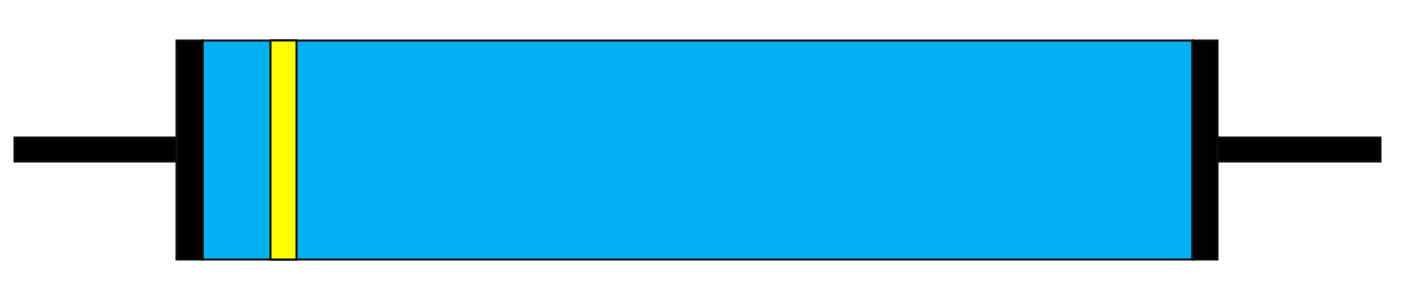
\includegraphics[width=0.7\textwidth]{2024/Abbildungen/Umkehrosmose/Entsalzen.png}
    \caption{Skizze zur Umkehrosmoseanlage}
\end{figure}

\newpage

\enumaufgabe{\operator{Berechne}, wie hoch die Konzentration $c$ von \ce{Na+} im Meerwasser ist und in dem aufgereinigten Wasser sein soll.}
\solution{
$$c_{\mathrm{Meer}}=\frac{n}{V}=\frac{\omega \rho}{M}=\frac{3,500\thinspace \% \cdot \SI{1025}{\kilogram\per\meter\cubed}}{\SI{58,44}{\gram\per\mole}}=\SI{0,6139}{M}\qquad \mathrm{1 P.}$$
$$c_{\mathrm{Trink}}=\frac{\beta}{M}=\frac{\SI{0,2000}{\gram\per\liter}}{\SI{22,99}{\gram\per\mole}}=\SI{8,699}{\milli\mole\per\liter}\qquad \mathrm{1 P.}$$
Insg. 2 P.}{4cm}




\enumaufgabe{\operator{Berechne} wie hoch der Druckunterschied mindestens sein muss, um aus den anfänglich \SI{5}{\liter} Meerwasser Trinkwasser zu machen. Gehe dabei von Standardbedingungen (\SI{0}{\celsius}, \SI{1}{\bar}) aus.\\
Falls du Teilaufgabe f) nicht oder nur teilweise gelöst hast, rechne mit $c_\mathrm{Meer}=0,7 \thinspace \mathrm{M}$ und $c_\mathrm{Trink}=0,01 \thinspace \mathrm{M}$.}

\solution{
Berechnung Menge Salz im Trinkwasser:
$$n(\ce{NaCl})_{\mathrm{Trink}}=V_{\mathrm{Trink}}\cdot c_{\mathrm{Meer}}=\SI{5,000}{\liter}\cdot\SI{0,6139}{\mole\per\liter}=\SI{3,070}{\mole}\qquad \mathrm{1 P.}$$
Daraus folgt ein endgültiges Volumen an Trinkwasser von:
$$V_\mathrm{Ende, Trink}=\frac{n(\ce{NaCl})_{\mathrm{Trink}}}{c(\ce{NaCl})_{\mathrm{Trink}}}=\frac{\SI{3,070}{\mole}}{\SI{8,699}{\milli\mole\per\liter}}=\SI{352,9}{\liter}\qquad \mathrm{1,5 P.}$$
ergo liegen dann noch $V_\mathrm{Ende, Meer}=\SI{405,0}{\liter}-\SI{352,9}{\liter}=\SI{52,1}{\liter}$ (1 P.) als hochkonzentriertes Meerwasser vor:
$$n(\ce{NaCl})_{\mathrm{Meer}}=V_{\mathrm{Meer}}\cdot c_{\mathrm{Meer}}=\SI{400,0}{\liter}\cdot\SI{0,6139}{\mole\per\liter}=\SI{245,6}{\mole}\qquad \mathrm{1 P.}$$
$$c_\mathrm{Ende, Meer}=\frac{n(\ce{NaCl})_{\mathrm{Meer}}}{V_\mathrm{Ende, Meer}}=\frac{\SI{245,6}{\mole}}{\SI{52,1}{\liter}}=\SI{4,714}{\mole\per\liter}\qquad \mathrm{1 P.}$$
Daraus folgt ein osmotischer Druck von:
$$\Pi=i\cdot \Delta c \cdot RT= 2\cdot (\SI{4,714}{\mole\per\liter}-\SI{8,699}{\milli\mole\per\liter})\cdot \SI{8,3145}{\joule\per\mole\per\kelvin}\cdot\SI{273,15}{\kelvin}=\SI{2,137e7}{\pascal}\qquad \mathrm{2,5 P.}$$
Da Druckunterschied wird $\Delta c$ betrachtet (1 P. von 2,5 P.) \\
Alternativergebnisse:\\
$n(\ce{NaCl})_{\mathrm{Trink}}=\SI{3,500}{\mole}$; $V_\mathrm{Ende, Trink}=\SI{350,0}{\liter}$; $V_\mathrm{Ende, Meer}=\SI{55,0}{\liter}$; $n(\ce{NaCl})_{\mathrm{Meer}}=\SI{280,0}{\mole}$; $c_\mathrm{Ende, Meer}=\SI{5,091}{\mole\per\liter}$; $\Pi=\SI{2,308e7}{\pascal}$\\
Insg. 8 P.}{12cm}

\solutiontext{$\sum$ 22 P.}{}
\end{document}
